% !TEX root = ../thesis.tex
\graphicspath{{./lyra/figures/}}
\chapter{A Visualization Design Environment (VDE)}

\begin{figure}[h!]
  \vspace{-40pt}
  \centering
  \includegraphics[width=\columnwidth]{playfair}
  \caption{The Lyra visualization design environment, here used to recreate William Playfair's classic chart comparing the price of wheat and wages in England. Lyra enables the design of custom visualizations without writing code.}
  \label{fig:lyra:teaser}
\end{figure}

Reactive Vega and Vega-Lite offer JSON syntaxes to facilitate programmatic
generation of interactive visualizations within higher-level interactive
applications. In this chapter, I explore this nascent space with Lyra: an
interactive visualization design environment (VDE). Lyra is motivated by
recognizing that Reactive Vega and Vega-Lite present a fundamental mismatch in
representations\,---\,using \emph{textual} languages to express \emph{visual}
output. As a result, with a commensurately poor ``closeness of
mapping,''~\cite{blackwell:cogdim} these languages impose a wide gulf of
execution~\cite{hutchins:directmanip}. It can be difficult for users to map
desired graphical outputs with the required textual specifications.

Existing graphical applications for visualization design, however, have limited
expressivity. At one end are \emph{chart typologies}~\cite{wilkinson:grammar}:
pre-defined palettes of chart types (bar charts, line charts, etc.) that make
numerous design decisions on behalf of the user. At the other end, vector
graphics packages offer designers complete flexibility but provide few (if any)
data-driven abstractions~\cite{bigelow:reflections}.

% !TEX root = ../thesis.tex
\section{User Interface Design}

Lyra was developed through an iterative user-centered design process. We held
formative interviews with representative users, such as visualization designers
and journalists, to understand their design process and the limitations of their
existing tools. These users evaluated low-fidelity prototypes and later
interactive prototypes.

The Lyra interface, as shown in \cref{fig:lyra:teaser}, is split into three
sections. The left-hand panel (\cref{fig:lyra:inspectors}(a)) depicts \emph{data
pipelines}: chains of data transformations applied to a data source. A
pipeline's inspector provides a paginated data table showing the output of the
pipeline, buttons to add new transformations, and a list of scales defined over
data fields. The right-hand panel (\cref{fig:lyra:inspectors}(c)) contains
inspectors for graphical elements such as marks, axes, and legends. These
elements are grouped into \emph{layers} to determine coordinate spaces and
z-ordering. These inspectors list all visual properties (position, fill color,
angle, etc.) along with widgets to manipulate them. The central panel contains
the visualization canvas where graphical elements may be directly manipulated.

\begin{figure}[t!]
\includegraphics[width=0.9\columnwidth]{inspectors}
\caption{Lyra's side-panels for data pipelines (left), and
visual properties (right). (a) Data table showing the current output
of the pipeline; (b) Scale transforms defined over fields in the pipeline.
(c) A property inspector for a symbol mark type; two properties have been
mapped to data fields.}
\label{fig:lyra:inspectors}
\end{figure}

\subsection{Data Pipelines}

Lyra's left-hand panel contains \emph{data pipelines}: workflows of transforms
applied to input data. Clicking a pipeline reveals an inspector that lists
applicable transforms and presents a paginated table view of transformed data.

\textbf{Data Table View}. Data pipelines include a data table view, using a
layout inspired by Bret Victor~\cite{victor:drawing}. The first column in the
table view lists field names, enabling vertical scanning. Subsequent columns
display individual records (\cref{fig:lyra:inspectors}(a)). Field names in the
first column are interactive: clicking a field sorts the table by that
dimension, drag-and-drop can be used to bind fields to mark properties. Fields
are colored by their source: green for fields in the original data and yellow
for fields derived by a transform. For example, the \emph{formula} transforms
adds new fields based on mathematical expressions. When \emph{group by}
transforms are applied, one tab for each group appears above the table view.

\textbf{Authoring Transforms}. Users can add a transform by clicking the
corresponding icon and configuring its parameters. Users may preview the effect
of applying a transformation in a popover. Once a transformation is added to the
pipeline, adjusting its properties is reflected in real-time across the table
view and the visualization.

\textbf{Scales}. The inspector also lists all scales defined over data fields in
the pipeline (\cref{fig:lyra:inspectors}(b)). Lyra automatically instantiates
scales when a field is associated with a mark property. The scale domain is
defined over the field values; the range is determined using production rules
described below. Users can also create scales manually. Users can drag scales
onto mark properties to apply a scale transform, or click a scale to access an
editor dialog (see \cref{fig:lyra:usage}(e)). When editing a scale that is not
represented by an axis or legend, a transient guide is shown in the canvas to
convey the effect of scale changes.

\subsubsection{Design Rationale}

Our initial prototypes hid raw data values in favor of exposing only the table
schema. However, evaluations indicated this was insufficient. Users noted that
it was difficult to determine the effect of a data transformation based solely
on the visualization. Moreover, the incremental nature of visualization design
can lead to unexpected intermediate output, for example setting the
\texttt{height} of a rectangle mark can cause all mark instances to overlap if
no \texttt{x} or \texttt{width} property has been set. Later prototypes
introduced a full data table view, to enable inspection of raw values and expose
the current data organization.

Similarly, early prototypes masked the presence of scales: mapping data to
visual properties automatically instantiated a scale, but they were not
explicitly exposed in the interface. When users attempted to construct
visualizations, we found that this significantly restricted their
expressiveness. For example, it is often necessary to specify custom ranges
for scales rather than rely on preset ranges. Such modification is difficult
to do without surfacing scales as a first-class construct. Later evaluations
found that users additionally had trouble identifying the purpose of scales,
or the effects of scale modification, if the scales were not explicitly
represented on the visualization by an axis or legend guide. In response, we
introduced transient guides.

\subsection{Composing Visual Elements}

Visualizations in Lyra are compositions of visual elements: graphical
\emph{marks} and \emph{guides}. Elements are grouped together into
\emph{layers}, which define local coordinates and establish z-ordering. Lyra's
right-hand panel lists the layers and their elements
(\cref{fig:lyra:inspectors}(c)). Elements are added to a visualization by
creating them within this panel or by dragging a mark from the mark palette.
When an element is selected, an inspector presents all the element's associated
properties. Property values may be edited directly or set via drag-and-drop of
data fields with changes reflected on the visualization in real-time. Hovering
over a property displays a guide overlaid on the visualization to illustrate how
that particular property affects the rendered output. Visual elements can also
be manipulated directly on the visualization canvas.

\begin{wrapfigure}{l}{0pt}
  \raisebox{0pt}[\dimexpr\height-1\baselineskip\relax]{\includegraphics
  [width=0.6cm]{handles}}
\end{wrapfigure}

\vspace{5pt}
\noindent
\textbf{Handles} in the canvas can be used to interactively move, rotate and
resize selected elements. A mark definition will typically render one mark
instance per datum in the visualization. To reduce visual clutter, selecting a
mark displays handles only on the instance that was clicked. However, when a
user adjusts the handles, the change is reflected simultaneously across all mark
instances.

\begin{wrapfigure}{l}{0pt}
  \hspace{-12pt}
  \raisebox{0pt}[\dimexpr\height-1\baselineskip\relax]{
  \includegraphics
  [width=1cm]{connectors}}
\end{wrapfigure}

\vspace{5pt}
\noindent
\textbf{Connectors} can be used to position marks relative to one-another.
Dragging a target mark onto a host mark's connector establishes a connection:
the target mark's position is now determined by the host's properties. Changes
to the host mark automatically propagate to all connected targets. Connectors
are particularly useful for positioning text labels relative to other marks.

\begin{wrapfigure}{l}{0pt}
  \raisebox{0pt}[\dimexpr\height-0.6\baselineskip\relax]{\includegraphics
  [width=2cm]{dropzones}}
\end{wrapfigure}

\vspace{5pt}
\noindent
\textbf{Drop zones} are used to associate data fields with mark properties. When
dragging a data field, drop zones are overlaid on the visualization canvas. Each
drop zone comprises a shaded region and a guide line or point to indicate the
corresponding mark property (e.g., \texttt{x}, \texttt{width}, etc.). Hovering
on a drop zone highlights it and shows the property name in a tooltip. Dropping
a field then establishes a mapping between the data field and the mark property.
To avoid clutter, Lyra shows drop zones only for the currently selected item.
When dragging a data field, users can hover and pause over a mark instance to
make it the selected item.

\subsubsection{Design Rationale}

Surfacing all properties in the inspector was an immediate first step to ensure
that Lyra maintained Vega's expressivity. Users noted that these inspectors were
akin to Tableau's ``shelves,'' a familiar interaction paradigm for many of them.
However, there remained a clear opportunity to further narrow the gulf of
execution~\cite{hutchins:directmanip} by pushing interactions to the
visualization canvas itself. For example, we observed users attempting to
select, move, or resize marks currently visualized on the canvas.

As users cited familiarity with drawing tools, we sought to reuse familiar
interaction mechanisms with \emph{handles} and \emph{connectors}. However, there
is not a similarly established interaction mechanism for data-property bindings.
We ultimately arrived at our \emph{drop zones} design by prototyping a number of
alternatives. One such alternative incorporated flow
menus~\cite{guimbretiere:flowmenu}. When dragging a data field over a mark on
the canvas, a flow menu would appear listing all mappable visual properties.
When dragging the field over a property, a submenu would appear listing
appropriate scale types given the type of the data field, and the particular
property. For example, for fields with numeric data, this submenu offered all
quantitative scale types including linear, logarithmic, and so forth. Dropping
the field over a particular scale type established a mapping and instantiated
the appropriate scale.

In addition to testing designs with users, we analyzed them using the Cognitive
Dimensions of Notation heuristics~\cite{blackwell:cogdim}. Data mapping through
flow menus, for example, provided a \emph{visible} and \emph{consistent}
interface---regardless of the mark type, all properties were consistently
ordered within the top-level menu. Although exposing scale types in the submenu
arguably reduced \emph{error\--proneness} (as Lyra need not infer a scale type),
it increased the \emph{diffuseness} (or verbosity) of the interface. User
feedback also revealed that selecting an option from this submenu was a
\emph{hard mental operation} as it forced them to select a particular scale type
up front. Many users perceived this as a \emph{premature commitment}. Perhaps
most troublesome, given our goal of reducing the gulf of execution, was the lack
of a \emph{closeness of mapping}: properties were listed as menu items, one
after another.

Drop zones, on the other hand, achieve a high \emph{closeness of mapping} as
they overlay the canvas in a way that corresponds to the property they
represent. For example, a rectangle's \texttt{x2} drop zone is shown extending
from the left edge of the canvas to the right-most edge of the rectangle.
Dropping a field over a drop zone performs \emph{scale inference} (described
below) to reuse an existing scale definition or instantiate a new one. Although
this may increase \emph{error-proneness}, it decreases \emph{diffuseness} and
reduces the \emph{hard mental operations} flow menus presented. One limitation
of drop zones is a subtle lack of \emph{consistency}; for example, a tall
rectangle mark will present a larger \texttt{height} drop zone than a shorter
one. We mitigate this issue by showing drop zones only for the currently
selected mark.

\subsection{Scale Inference and Production Rules}

When a user binds a data field to a mark property, Lyra performs \emph{scale
inference} in an attempt to reuse existing scale definitions. Lyra searches for
an existing scale with the field as its domain. If a scale is found, it is
reused if its range type is appropriate (e.g., spatial or color values). If no
scale is found or the range type does not match, Lyra instantiates a new scale:
ordinal for categorical data or linear for quantitative data, along with a
default range based on the property type (e.g. \texttt{width} for \texttt{x}
properties).

To accelerate common encoding decisions, Lyra also uses a set of context- and
mark-specific \emph{production rules} to determine intelligent defaults. These
production rules may set additional properties of the mark or add new graphical
elements to the canvas. For example, dropping a field over a rectangle mark's
\texttt{width} drop zone automatically binds the \texttt{x} property as well to
correctly position each rectangle. Dropping a field over a spatial property may
add an axis; dropping a field over a color property may add a legend. A user can
customize these defaults using the property inspector. However, users may
occasionally wish to sidestep the production rules. Accordingly, Lyra evaluates
production rules only when a mapping is established using drop zones. If the
user instead drops a data field onto the property inspector panel, no production
rules are evaluated and so no defaults are added.

\subsubsection{Design Rationale}

Scale inference and production rules were informed primarily by early user
feedback. Without these features, users had to manually create every aspect of
the visualization, which they found to be tedious. Users did not expect to have
to specify a scale definition on every data mapping operation, and expected axes
or legends to be automatically added as appropriate. We found that the features
did alleviate this tedium but, interestingly, users subsequently requested a
method of circumventing them \emph{``if they knew better''}. As a result,
although Lyra performs scale inference on every data field mapping, production
rules are only evaluated if the data field is dropped over a drop zone. Users
may sidestep the rules by working directly with property inspector instead. We
fully enumerate Lyra's scale inference procedure and production rules in
supplementary material.

\subsection{Saving and Exporting Visualizations}

Visualizations built in Lyra can be exported as static PNG or SVG files, or as
Vega JSON specifications. With Vega's JavaScript runtime, the JSON file can be
parsed and rendered on a web page, dynamically bound to new input data, and
extended with interactions using JavaScript event callbacks. Vega specifications
optionally can contain both input data and visual encoding directives, providing
a single standalone file for sharing a visualization instance.
% !TEX root = ../thesis.tex
\section{Implementation Details}

Lyra is a web-based HTML5 application built using
AngularJS\footnote{http://angularjs.org}. Vega is used extensively throughout
the system both to parse data transformations and to represent and generate
visualizations. While close, the mapping between Lyra and Vega abstractions is
not one-to-one. To reduce complexity, Lyra consolidates some Vega mark types. A
line mark in Lyra translates to one of Vega's line, path, or rule marks based on
which properties and fields the designer chooses to map. Similarly, Vega's image
marks are simply rectangle marks in Lyra with an ``image fill.''

Lyra also simplifies Vega's handling of hierarchical data. In a Vega
specification, each level of a hierarchy is assigned to a ``group'' mark, with
children marks inheriting the corresponding subset of data. Lyra insulates users
from this scheme by automatically performing \emph{group injection}: when a user
assigns a mark to a pipeline containing hierarchical data, Lyra automatically
adds and nests the necessary group marks for each level of the hierarchy in the
resulting Vega specification. Group injection makes building small multiples
easy: an exposed \texttt{layout} property lets designers choose between having
groups overlap, layout horizontally, or layout vertically.

Lyra's direct manipulation interactors (handles, connectors, drop zones) are
also generated using Vega, using a separate specification rendered \emph{over}
the visualization. The geometry of the marks serves as input data for this
interactive layer. By decoupling the visualization and interactors, we ensure
that Lyra features do not interfere with the designer's visualization.
% !TEX root = ../thesis.tex
\section{Usage Scenario}

\emph{Dissecting a Trailer}~\cite{nytimes:trailer} is a visualization from The
New York Times that illustrates how scenes from five Best Picture Oscar nominees
were edited into trailers. It is an example of a visualization that cannot be
built using existing chart typologies or high-level grammars. The visualization
layers several mark types and uses a non-standard ``scatter'' plot with small
rectangles of varying widths. The original consists of over 350 lines of
JavaScript/D3~\cite{bostock:d3} code. Here, we demonstrate how this graphic can
be created using Lyra (Fig.~\ref{fig:lyra:usage}).

\begin{figure}[h!]
\floatbox[{\capbeside\thisfloatsetup{capbesideposition=
{right,center},capbesidewidth=0.3\columnwidth}}]{figure}[\FBwidth]
{\caption{Using Lyra to recreate the New York Times' Dissecting a Trailer.
(a)~Drag a line \emph{mark} onto the canvas. (b)~Drag a field from a
\emph{pipeline}'s data table to a \emph{drop zone} to map it to a mark property.
(c)~Add a ``group by'' \emph{data transform} to create a hierarchy. (d)~Edit a
\emph{scale} definition to reverse the range. (e)~Use a \emph{connector} to
anchor text marks to the rectangles.}
\label{fig:lyra:usage}}
{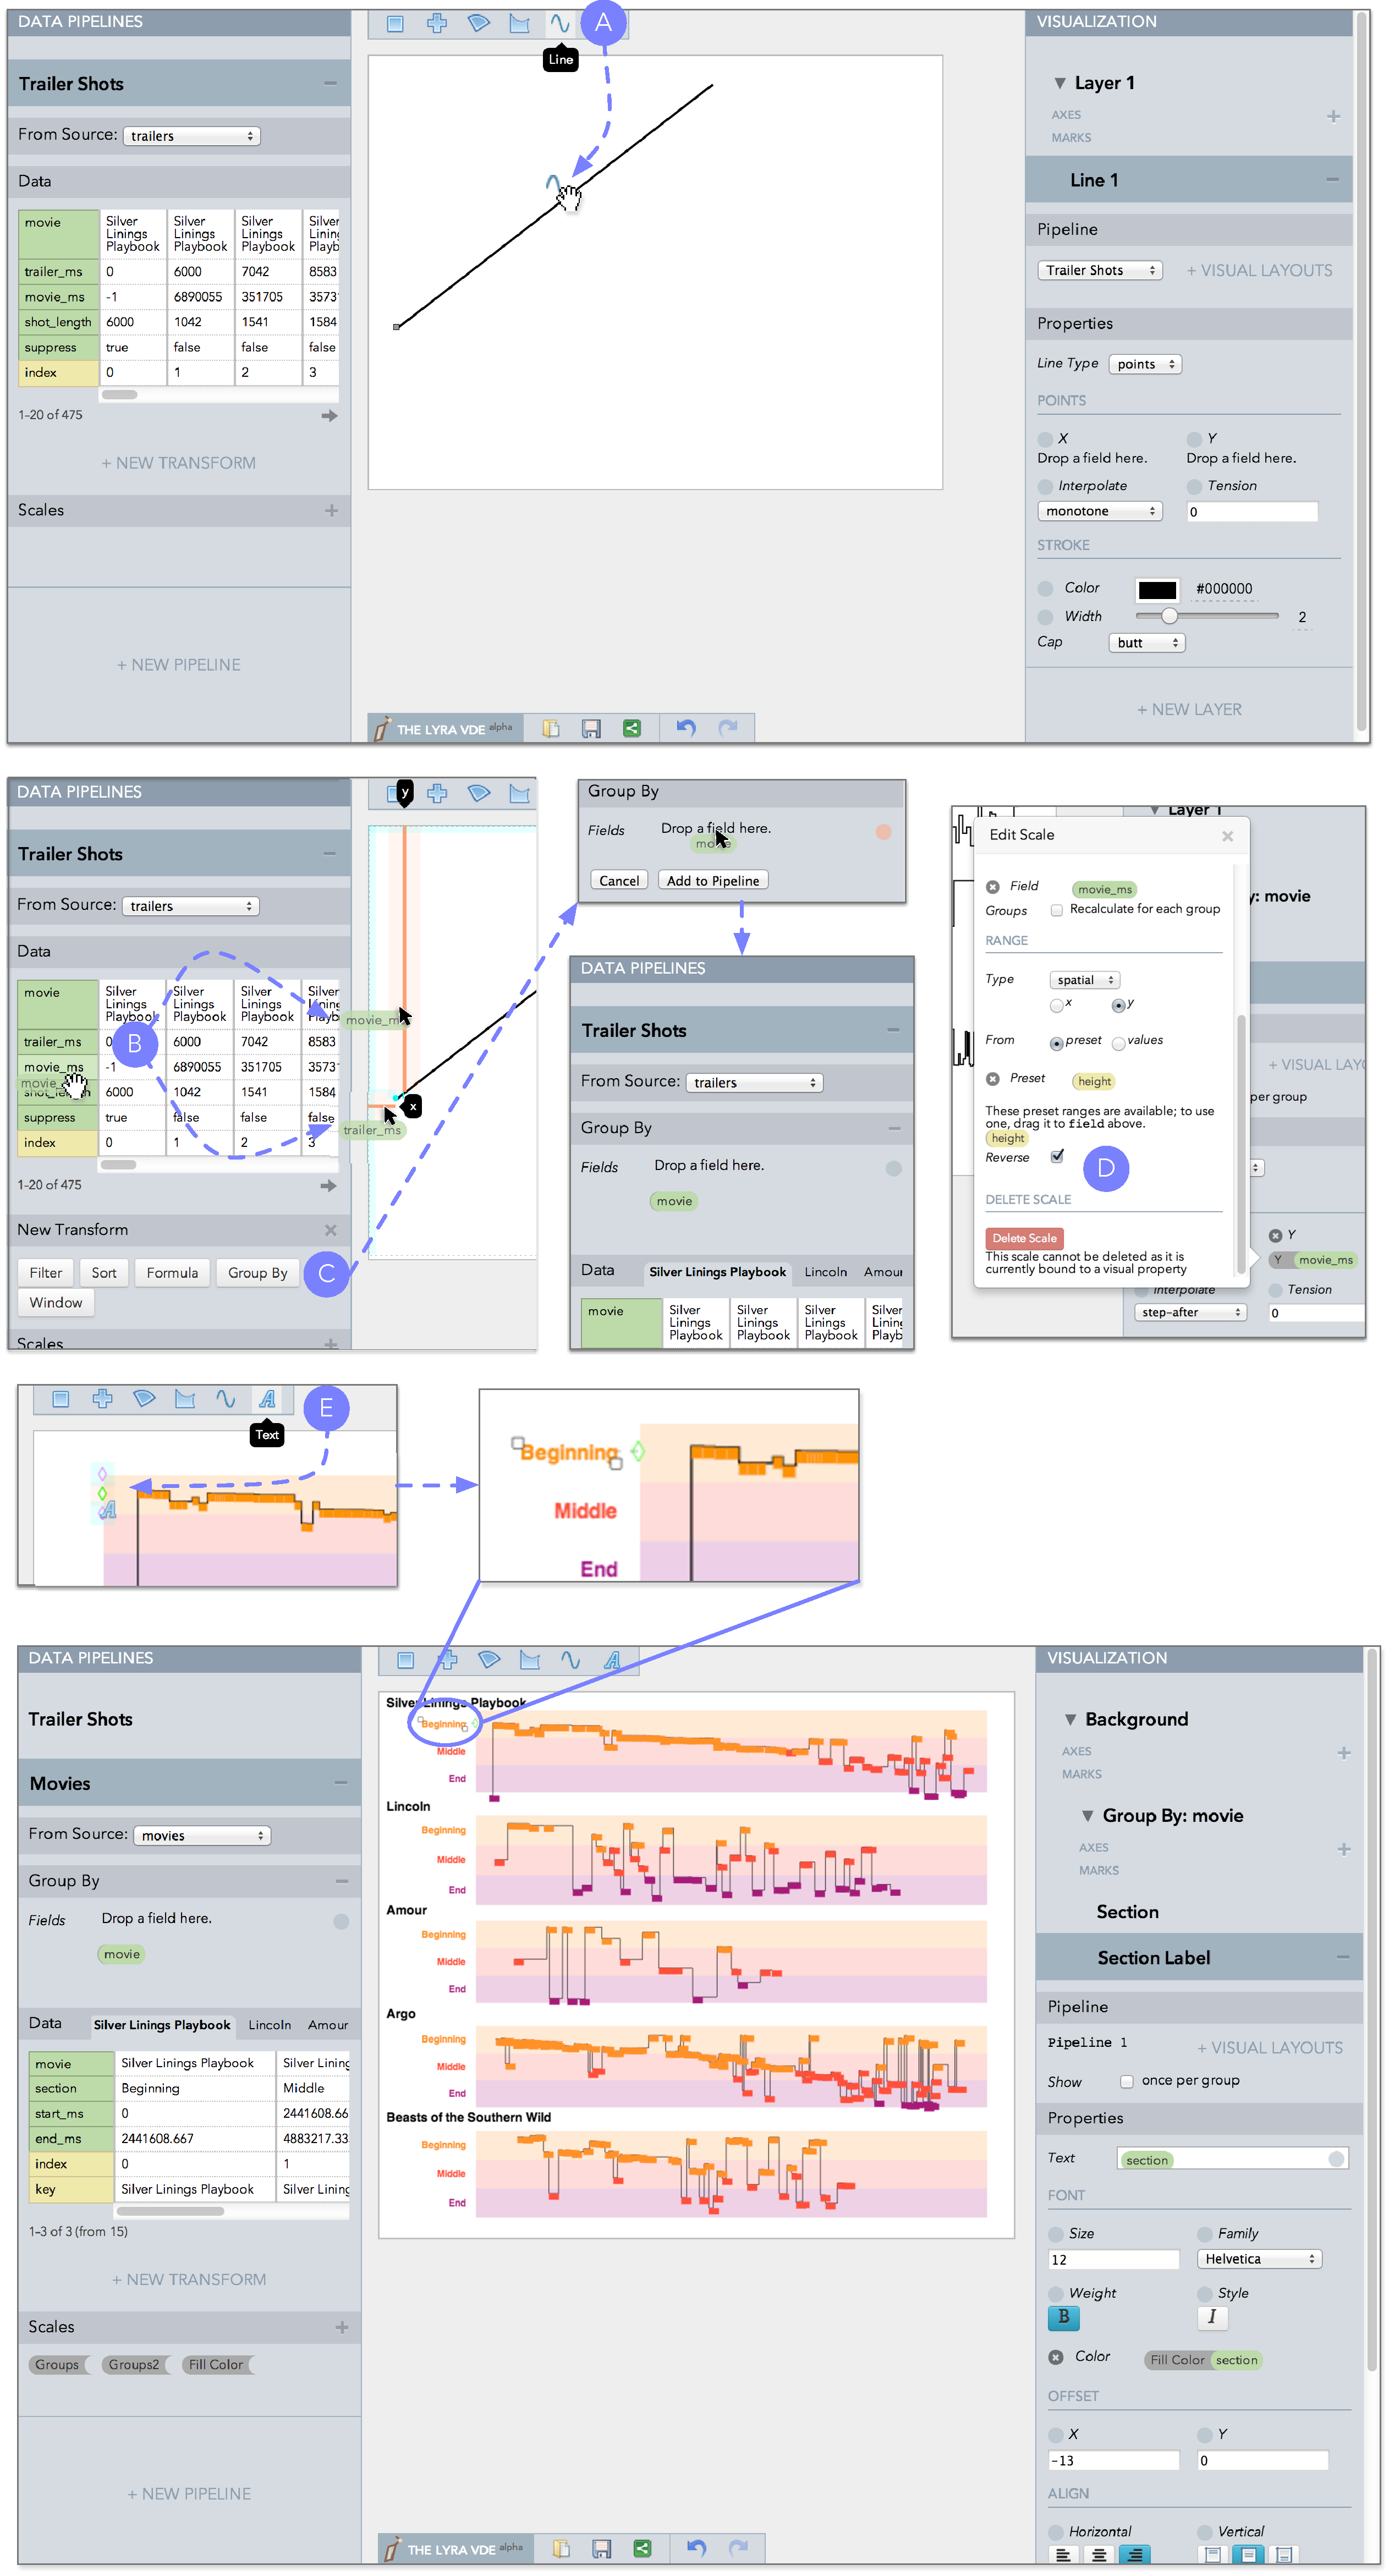
\includegraphics[width=0.7\textwidth]{usage}}
\end{figure}

We introduce lines by dragging a \emph{line mark} from the palette at the top of
the screen and dropping it on the canvas (Fig.~\ref{fig:lyra:usage}(a)). This
adds a new line (backed by a single datum) to the current layer and associates
it with a new data pipeline. The default pipeline is empty, as we have not yet
specified a data source. To register a new source, we provide a name and a URL
to our trailer shots data, and, upon load, review the inferred data types
(number, string, etc.) for each data field. The output of the pipeline is then
shown in the data table at the bottom of the pipeline inspector
(Fig.~\ref{fig:lyra:usage}(b)).

We bind data in the pipeline to visual properties of the line mark via
drag-and-drop of data fields. Dragging triggers the display of \emph{drop zones}
overlaid on the visualization canvas. Dropping a data field on a zone
establishes a visual encoding (Fig.~\ref{fig:lyra:usage}(b)). We drag
\texttt{trailer\_ms} and drop it over the line's \texttt{x} property, then drop
\texttt{movie\_ms} over \texttt{y}. These actions result in line segments
connecting every data point.

However, we desire separate line charts per film. To divide the data, we add a
\emph{group by} transformation to our pipeline (Fig.~\ref{fig:lyra:usage}(c)),
keyed on the movie title. The data table reflects the result via tabbed groups,
and the mark's property inspector now offers an option for group
\texttt{layout}. We choose a \texttt{vertical} layout to produce one line per
movie, arrayed down the canvas. We now see that the data includes shots that
appear in trailers but not in movies (identified by the \texttt{suppress}
field); we add a \emph{filter} transform to remove them
(Fig.~\ref{fig:lyra:usage}(d)). Next, we want film timelines oriented
top-to-bottom, but our lines show the reverse. We adjust the orientation of the
y-axis \emph{scale} by reversing its scale range (Fig.~\ref{fig:lyra:usage}(e)).

Next, we add small rectangle plots by dragging a \emph{rectangle mark} onto the
canvas. Lyra automatically associates the mark with the current pipeline and the
visualization now shows one rectangle per shot. As with the line mark, we drag
\texttt{trailer\_ms} and \texttt{movie\_ms} to the rectangle's \texttt{x} and
\texttt{y} property drop zones. We size the rectangles by dragging
\texttt{shot\_length} over the \texttt{width} drop zone and dragging the bottom
\emph{handle} to manually set the desired height (Fig.~\ref{fig:lyra:usage}(f)).
To color rectangles based on shot onset time in the film, we drag
\texttt{movie\_ms} over the \texttt{fill} property drop zone, and choose custom
colors in the resulting scale definition dialog.

The final step is to create labels and background rectangles to identify the
movies and their beginning, middle, and end sections. As these elements should
reside in the background, we create a new layer in Lyra. Movie section
information is drawn from a different data source, so we create a new pipeline.
We then drag a rectangle mark onto the canvas, and drag the section
\texttt{start} and \texttt{end} fields onto the rectangle \texttt{y} and
\texttt{y2} properties, resulting in a vertical layout for beginning, middle,
and end sections. We bind the \texttt{label} field to the fill color property
and select custom colors for the resulting scale mapping. To label each section,
we drag a \emph{text mark} from the palette and drop it on a rectangle's
diamond-shaped \emph{connector} (Fig.~\ref{fig:lyra:usage}(g)). Doing so anchors
the text mark coordinates to the rectangle. Finally, we bind the \texttt{label}
field as textual content and set the text fill color. We now can export the
visualization as either a Vega specification or an image file.
% !TEX root = ../thesis.tex
\vspace{-10pt}

\section{Example Visualizations}

\vspace{-10pt}

One of Lyra's primary goals is to enable an expressive design space. With Lyra,
it should be possible to create visualizations that would have previously
required programming. To assess the extent to which this goal has been met, we
constructed a diverse collection of example visualizations, including those
shown below. These examples compose multiple mark types, and many require
multiple data pipelines. For example, Fig.~\ref{fig:lyra:caltrain} uses line,
symbol, and text marks to convey two datasets: train routes and stations.
Fig.~\ref{fig:lyra:bertin} demonstrates that Lyra's integration of data
pipelines and graphical manipulation is necessary to maintain expressiveness:
shading the bars requires a data pipeline with \emph{Group By} and
\emph{Formula} data transformations applied.

Similarly, exposing visual layout inspectors allows for rapid design iteration.
In Fig.~\ref{fig:lyra:les_mis}, for example, the \emph{force-directed layout}
inspector exposes parameters such as link distance, strength and gravity;
adjusting them re-renders the layout in real-time. The layout also augments
direct manipulation on the canvas: designers can brush to select nodes and
double-click to pin them. Together, these facilitate a converging process:
pinning satisfactory nodes, adjusting layout properties, and re-running the
layout to reposition unpinned nodes. This process would be cumbersome using only
D3's force-directed layout~\cite{bostock:d3}: after programming the layout,
adjusting parameters requires editing the code and refreshing the browser.
Pinning nodes then requires inspecting the properties of each rendered node
individually and copying the \texttt{x} and \texttt{y} positions into the raw
dataset.

\begin{figure}[h!]
  \centering
  \includegraphics[width=\columnwidth]{bullet_chart}
  \caption{Bullet chart using rectangle and symbol marks grouped
by category. Labels are positioned via a left-edge connector on rectangles.}
  \label{fig:lyra:bulletChart}
\end{figure}

\begin{figure}[h!]
  \centering
  \includegraphics[width=\columnwidth]{driving}
  \caption{A recreation of \emph{Driving Shifts Into Reverse} by Hannah
  Fairfield from The New York Times, originally published May 2, 2010.}
  \label{fig:lyra:gas_driving}
\end{figure}

\begin{figure}[h!]
  \centering
  \includegraphics[width=\columnwidth]{les-mis}
  \caption{Character co-occurrences in Les
Mis\'{e}rables. Colors represent cluster memberships computed by a
community-detection algorithm.}
  \label{fig:lyra:les_mis}
\end{figure}

\begin{figure}[h!]
  \centering
  \includegraphics[width=\columnwidth]{caltrain}
  \caption{The schedule of the San Francisco Bay Area's CalTrain service in the style of E. J. Marey's Paris train schedule.}
  \label{fig:lyra:caltrain}
\end{figure}

\begin{figure}[h!]
  \centering
  \includegraphics[width=\columnwidth]{zipscribble}
  \caption{ZipScribble by Kosara~\cite{kosara:zipscribble}. A \emph{geo} layout
 encoder is used with line marks to connect latitude and longitudes of zip
 codes.}
  \label{fig:lyra:zipscribble}
\end{figure}

\begin{figure}[h!]
  \centering
  \includegraphics[width=\columnwidth]{streamgraph}
  \caption{A streamgraph of unemployed U.S. workers by industry, using a
  \emph{stack} layout with a \texttt{wiggle} offset~\cite{byron:streamgraph}.}
  \label{fig:lyra:streamgraph}
\end{figure}

\begin{figure}[h!]
  \centering
  \includegraphics[width=\columnwidth]{napoleon}
  \caption{Minard's map of Napoleon's Russian campaign. A \emph{geo} transform
 encodes spatial positions; army size maps to line stroke width.}
  \label{fig:lyra:napoleon}
\end{figure}

\begin{figure}[h!]
  \centering
  \includegraphics[width=\columnwidth]{bertin}
  \caption{Jacques Bertin's analysis of hotel patterns. \emph{Group by} and \emph{formula}
 transforms are used to shade bars with values above the mean.}
  \label{fig:lyra:bertin}
\end{figure}

\clearpage

\subsection{Limitations}

\vspace{-7pt}

\Cref{fig:lyra:usage,fig:lyra:bulletChart,fig:lyra:gas_driving,fig:lyra:les_mis,fig:lyra:caltrain,fig:lyra:zipscribble,fig:lyra:streamgraph,fig:lyra:napoleon,fig:lyra:bertin}
demonstrate that Lyra enables an expressive design space, but creating these
examples also reveals some limitations. Vega currently lacks support for polar
coordinates. As a result, Lyra cannot (yet) provide \emph{arc} mark connectors
or produce radial axes, making it difficult to recreate classic visualizations
such as Nightingale's Rose or Burtin's antibiotics chart. Additionally, Lyra
only supports the \textsc{rgb} color space, while Vega also supports
\textsc{hsl}, \textsc{lab}, and \textsc{hcl}. These color spaces facilitate
perceptually-sound designs. We plan to address these limitations in future
versions of Vega and Lyra.
% !TEX root = ../thesis.tex

\vspace{-10pt}

\section{Formative User Evaluations}

\vspace{-10pt}

Lyra was designed to support both expressive and \emph{accessible} visualization
design: users should not require coding expertise to be able to construct custom
visualizations. To evaluate Lyra's accessibility, we conducted first-use studies
with 15 representative users including 6 data analysts / visualization
designers, 5 data journalists, and 4 graduate students in data visualization. On
10-point scales, the median self-reported visualization design expertise was 7,
while programming expertise range between 2--8. These users all use
visualization as a communicative medium but their processes for creating them
vary. The visualization designers and grad students were more technically
proficient and typically use D3, whereas the data journalists rely on chart
typologies (Microsoft Excel) or grammar-based systems (Tableau) that do not
require programming. Some journalists also reported eschewing visualization
systems in favor of drawing programs such as Adobe Illustrator.

\vspace{-10pt}

\subsection{Methods}

\vspace{-7pt}

We began each study with a 10 minute tutorial. We then asked participants to
design three graphics: a bar chart of medal count by country at the 2012
Olympics (T1), a grouped or stacked bar chart of medal counts by medal type and
country (T2), and a trellis plot of barley yields (T3,
Fig.~\ref{fig:lyra:trellis}). These tasks were designed to ensure participants
interacted with all aspects of Lyra. Each task was more difficult than the
previous, intending to first familiarize participants with the Lyra design
process, and then challenge them. Participants were encouraged to think-aloud
and were de-briefed at the end. Sessions lasted approximately 45 minutes, after
which we administered a post-study survey.

\begin{figure}[b!]
  \centering
  \includegraphics[width=1\columnwidth]{barley}
  \caption{Study participants recreated the barley yields Trellis
  display~\cite{becker:trellis}.}
  \label{fig:lyra:trellis}
\end{figure}

\vspace{-10pt}

\subsection{Successes}

\vspace{-7pt}

Users quickly learned Lyra's interaction model and all users, regardless of
their technical expertise, successfully completed all three tasks with minimal
guidance (100\% task completion rate). Users completed the first two tasks in
just a few minutes, the more complex third task took longer (T1: median time =
1:33, inter-quartile range (IQR) = 0:51; T2: median = 2:43, IQR = 2:57; T3:
median = 10:24, IQR = 4:00). In a post- study survey, users rated Lyra's
interface highly: drop zones felt natural to use ($\mu$ = 4.4, $\sigma$ = 0.57
on a 5-point Likert scale), connectors helped to relatively position marks
($\mu$ = 4.3, $\sigma$ = 0.49), and a pipeline's data table helped evaluate
context ($\mu$ = 4.4, $\sigma$ = 0.51). Handles were found useful for resizing
and positioning ($\mu$ = 3.8, $\sigma$ = 0.45) but users noted that the
properties they control are typically mapped to data. When asked to recount
their experience, users described drop zones as \emph{``natural''} and
\emph{``intuitive.''} One user stated, ``\emph{it's like \emph{literally} saying
`put that there.'}'' Others drew comparisons to Tableau's shelves:
\emph{``[shelves] don't always behave like I expect them to but [drop zones]
make me feel more in control.''} One participant ended his session by saying
that \emph{``there's a real joy in using Lyra.''}

Two journalists who participated lead data visualization teams in their
organizations. They appreciated that Lyra took cues from familiar drawing tools.
They welcomed Lyra's image export options, particularly SVG export, as the
visualizations they produce are often reutilized in print media. One suggested
that Lyra could be a powerful training tool that could help familiarize his team
with the process of designing visualizations from the ground-up.

\begin{figure}[b!]
\centering
  \includegraphics[width=\columnwidth]{sara}
  \caption{A study participant approximately recreated a D3 visualization (left,
  requiring 4-6 hours) in Lyra (right, requiring only 10 minutes).}
  \label{fig:lyra:sara_waitlists}
\end{figure}

Users familiar with lower-level tools such as D3 found Lyra useful for rapidly
prototyping and iterating on their design. For example, one user (self-rated
expertise with D3 as 6.5/10) used Lyra with her own data. By her estimate, she
had previously spent between 4--6 hours repurposing an existing D3 example to
create a custom visualization. She was able to create a close approximation in
Lyra, shown in \cref{fig:lyra:sara_waitlists}, in only 10 minutes.

\subsection{Shortcomings}

We also observed that Lyra posed certain challenges for our participants.
Although users found drop zones natural and intuitive, they noted problems with
the current implementation. First, when users missed a drop zone by a few
pixels, they expected Lyra to infer their intent. Second, when users
successfully dropped a field, they would lose track of the currently selected
mark if it was repositioned. A third shortcoming was Lyra's lack of support for
undo, which led users to become more hesitant to freely explore. Undo support
has since been added to Lyra, and we plan to address the remaining issues in
future versions. For example, a Voronoi diagram could be used to find the
nearest drop zone~\cite{grossman:bubble}, and staggered animated transitions
could help users better track changes~\cite{heer:animated} to marks.

Finally, several users mentioned that learning from and repurposing existing
visualizations is an important part of their design process. They found the
blank canvas to be an intimidating starting point. We anticipate that
providing a gallery of examples (including those in this paper) that users can
import, reuse and modify would mitigate this issue.

% !TEX root = ../thesis.tex
\vspace{-10pt}

\section{Reflections \& Future Work}

\vspace{-10pt}

\begin{figure}[b!]
\includegraphics[width=\columnwidth]{lyra2}
\caption{The new Lyra interface. The side panels from \cref{fig:lyra:inspectors}
have been redesigned and consolidated to the left-hand side. As the user drags a
data field across the canvas, the nearest drop zone (highlighted in orange) is
automatically selected\,---\,a technique known as a bubble
cursor~\cite{grossman:bubble}.}
\label{fig:lyra2}
\end{figure}

Chronologically, Lyra was the first project to form part of this dissertation.
At the time of writing, a new version, that leverages Reactive Vega and
Vega-Lite, is under development. Thus, it is worth reflecting on how its role in
the ecosystem has evolved.

Much of Lyra's existing functionality can now be driven purely via a Reactive
Vega specification rather than through external callbacks. For instance, direct
manipulation operations on handles are now driven entirely via signals, rather
than event handling callbacks. Similarly, connectors make use of reactive
geometry directly. A bubble cursor~\cite{grossman:bubble} UDF (see
\cref{sec:udfs}) is registered to accelerate drop zone selection, as shown in
\cref{fig:lyra2}, addressing a major shortcoming users identified previously.

Moreover, Lyra's built-in production rule system has been subsumed by Vega-Lite.
Now, when users drag a data field onto a drop zone, a Vega-Lite unit
specification is compiled, the resultant Vega specification is statically
analyzed, and components selectively merged or updated in Lyra's backing Vega
specification.

With these changes, Lyra's place in the tool stack comes into sharper relief: it
\emph{bridges} two levels of abstraction within a single, cohesive environment.
Direct manipulation operations occur at the Vega-Lite level, and allow users to
rapidly generate recognizable visualizations. For more fine-grained
manipulation, or for custom design elements, users drop down to the Vega level
by interacting with the visual inspectors. A critical advantage of this approach
is that users can fluidly work with the level of abstraction best suited for the
task at hand. In fact, they may be altogether unaware of the separate roles
played by Vega and Vega-Lite under-the-hood!

Looking ahead, an exciting challenge is how Lyra might be extended to support
the design of \emph{interactive} visualizations. In-keeping with the above
approach, perhaps direct manipulation interactions (or demonstrations) should
generate Vega-Lite selections, which can be further modified with signal and
predicate inspectors.

Similarly, while Lyra's primary focus is currently on design tasks, data
visualization inevitably requires data cleaning and transformation. Lyra's data
pipelines offer sufficient flexibility to support analytic tasks, but require
familiarity with transformation operators. Can direct manipulation methods, akin
to those in Data Wrangler~\cite{kandel:wrangler}, be further incorporated to
specify more complex data transformations?